\documentclass[a4paper]{article}

\usepackage{amsmath,amsthm,amssymb}
\usepackage{tikz}
\usetikzlibrary{external}
\tikzexternalize[prefix=figures/]

\tikzset{
every node/.style={circle, draw, inner sep=2pt},
every label/.style={rectangle, draw=none}
}

\begin{document}

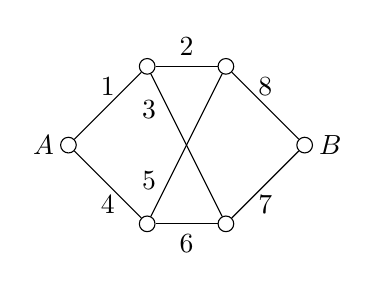
\begin{tikzpicture}
\node[label={left:$A$}] (0)  at (0,0) {};
\node (1)  at (1,1) {};
\node (2)  at (1,-1) {};
\node (3)  at (2,1) {};
\node (4)  at (2,-1) {};
\node[label={right:$B$}] (5)  at (3,0) {};

\draw (0) --node[midway,above,draw=none] {$1$} (1);
\draw (0) --node[midway,below,draw=none] {$4$} (2);
\draw (1) --node[midway,above,draw=none] {$2$} (3);
\draw (1) --node[near start,left,draw=none] {$3$} (4);
\draw (2) --node[near start,left,draw=none] {$5$} (3);
\draw (2) --node[midway,below,draw=none] {$6$} (4);
\draw (3) --node[midway,above,draw=none] {$8$} (5);
\draw (4) --node[midway,below,draw=none] {$7$} (5);

\end{tikzpicture}


\end{document}


%%% compile by pdflatex --shell-escape filename.tex
